\chapter{TinyFuncCoder}
\label{chap:tinycoder}
This chapter presents the contributions made by this thesis, namely the TinyFuncCoder series of \acp{lm} as well as the TinyFuncData dataset.
It explains the dataset creation in section \ref{sec:data}, model architecture in section \ref{sec:architecture} and the training and evaluation processes in sections \ref{sec:training} and \ref{sec:eval} respectively.
A link to the source code is provided in section \ref{sec:repo} alongside an explanation of the repository structure.
Most work in the following sections was done using Jupyter Notebooks\footnote{\url{https://jupyter.org/} (last visited on 2024-10-31)}, a common tool for working with \acp{lm} and data science in general.

\section{Dataset Creation}
\label{sec:data}

This section will describe the process for gathering and preparing the TinyFuncData dataset used to train the TinyFuncCoder series.
The starting point for dataset creation was the deduplicated version of The Stack dataset \cite{Kocetkov.2023}.
It consists of 3 TB of open source GitHub files spread among 358 programming languages.
Further details about this dataset are explained in section \ref{sec:thestack}.

The dataset was loaded into the notebook using \texttt{load\_dataset} from huggingface's \texttt{data}-\texttt{sets} package, using the \texttt{streaming=True} option, which prevents the whole dataset from being downloaded at once, but rather loading it into memory in chunks.
This is done to limit the storage cost of working with large datasets such as The Stack.

Of the columns included in The Stack, the ones used in data extraction were
\begin{itemize}
    \item \texttt{hexsha}: A unique git hash, used as an id
    \item \texttt{lang}: The language of the file
    \item \texttt{max\_stars\_count}: The number of stars of the repository
    \item \texttt{content}: The code in the file
\end{itemize}

Two filters were applied to the dataset:
First, only GitHub's top ten languages as of Q4 2023 were kept \cite{GitHub.2024}, excluding Makefile and Dockerfile as they do not support functions.
To replace them, C\# and Ruby, the languages in 11th and 12th place, were included.
GitHub's top languages were chosen as the data from The Stack is also gathered from it.
As the model is mainly aimed at students, a lot of programming languages are a low priority or entirely obsolete for training.
Instead, focus should be set on the most popular programming languages with which they are most likely to interact.
The language count is set to ten to have a varied amount of popular languages while keeping the scope of the data limited.
Loading the data was done using the \texttt{data\_dir} parameter to stream only the data of each language individually, reducing the amount of data that must be processed drastically.
Next, any file from a repository with a ranking of lower than three stars was excluded.
Stars indicate that the repository has been marked as a favorite and measure popularity.
Three stars is set to exclude repositories with little to no traction.

The next step was to extract all function definitions out of all code files of each language, including the function head, body, and optionally parameters and a docstring.
This is done to train TinyFuncCoder on pure function definitions -- training it on whole code files would introduce overarching knowledge of class or file structures which is not desired.
To extract function definitions, every language had to be treated individually.

\paragraph{Python} was the easiest language to filter.
Since all of the preparation was done in a jupyter notebook, the Python library \texttt{ast} could be used to parse python code from a string into an \ac{ast}.
This \ac{ast} object has built-in functionality to extract all above listed attributes of all functions in a given file.

For all other languages, a \ac{regex} was written to extract the functions from the content string.
\Ac{regex} is a structured language used in pattern recognition and extraction of these patterns from strings.

\paragraph{Languages with a function keyword} including PHP (\texttt{function}), JavaScript (\texttt{function}) and TypeScript (\texttt{function}), but excluding Ruby (\texttt{def}), which will be filtered uniquely, were straightforward to parse, as the \ac{regex} can center around the keyword and be certain to only capture functions.
For example, the \ac{regex} for PHP looks as follows:

\begin{verbatim}
(?<doc>(?:\/\*\*.*?\*\/|\/\/.*?\n)?)\s*

(?<name>(public|protected|private)*\s*function\s+\w+)\s*

(?<args>\((?:[^()]+|(?&args))*\))\s*

(?<body>\{(?:[^{}]+|(?&body))*\})
\end{verbatim}

This regex is seperated into the groups \texttt{(?<doc>)}, \texttt{(?<name>)}, \texttt{(?<args>)} and \texttt{(?<body>)}, corresponding to the four desired elements to extract.
The regex is applied as a whole, with the linebreaks only serving to show each group individually and aiding readability.
Each group besides the last is also capped with optional whitespaces (\texttt{$\backslash$s*}).

The doc group captures a docstring by looking for the start and end of a multiline comment (//* \dots */) or a one-line comment and line break (\texttt{// \dots $\backslash$n}). It is marked as optional with a question mark, as a docstring is not necessarily given.

The name group captures the function definition up to the parameters, including an optional access modifier (\texttt{public}, \texttt{protected} or \texttt{private}), the word \texttt{function} and any user-given name (\texttt{$\backslash$w+}).

The args group captures all arguments given, starting with the opening bracket after the function name and ending with the closing bracket just before the opening curly bracket for the body.
It is the first group where a recursive search has to be done to match an open bracket to the same closing bracket.
This has to be done as if there is a closing bracket anywhere within the parameter list, the \ac{regex} will assume that it ends at that point.
For this reason, all open-close bracket pairs have to be detected, and it must be assumed that the code is well formed (meaning that all opening brackets have to have a closing bracket).
To do this, a recursive block is used that matches either any character that is not an opening or closing bracket, or if a bracket is found, a recursive search of the same pattern within that bracket up to the next closing bracket.
As a function may not have parameters, only one set of brackets is necessary for the function declaration.

Finally, the body group captures the function body from the opening curly bracket to the corresponding closing bracket.
This syntax also requires a recursive search, even moreso than the args block, as the body is much more likely to contain opening and closing brackets within itself, for any nested blocks like \texttt{if}s, \texttt{while}s and more.
These two recursive searches also necessitate the naming of the blocks, as they should be recursively searched individually, not the entire pattern including the docstring and name.

The other two languages require mild variations depending on language specifics but look mostly the same.

\paragraph{Languages without a function keyword} including C, C++, C\#, Java and Shell are slightly more complicated to parse, while functioning broadly the same as the previous group.
The main difference is the name block, as it cannot center around a keyword.
For Java, the \ac{regex} looks as follows:

\begin{verbatim}
    (?<doc>(?:\/\*\*.*?\*\/|\/\/.*?\n)?)\s*
    
    (?<name>(?:public|private|protected)?\s*(?:static)?\s*\w+\s+\w+)\s*
    
    (?<paren>\((?:[^()]+|(?&paren))*\))\s*
    
    (?<brace>\{(?:[^{}]+|(?&brace))*\})
\end{verbatim}

Besides the slightly altered access modifiers, the name is now matched as two words, namely a return type and a user-given name (the easiest example would be \texttt{public static void main}).

This \ac{regex} pattern also matches certain blocks of code that are not function definitions, such as an if-else block -- \texttt{if else (\dots) \{\dots\}} also matches the word-word-args-body pattern.
To combat this, the captured functions then check their name against a list of keywords, removing those that exactly match keywords from these languages.
As keywords are banned from verbatim use as user-defined names, this will filter out all undesired matches without removing real functions.
The regex for the other languages works similarly, with minor adjustments for language specific syntax.

\paragraph{Ruby} was the most complex language to parse as it is the only one besides Python that does not use curly brackets to open and close blocks, without having the benefit of a library like \ac{ast}.
This means Ruby files have to be prepared before they can be given to the \ac{regex}.
As Ruby also uses a function keyword (\texttt{def}), the easiest way to prepare it is to simply insert curly brackets next to all keywords that start and end code blocks and then apply a \ac{regex} like the one already defined.
All keywords that open a block like \texttt{do}, \texttt{class} or \texttt{if} are given an opening bracket directly after the word.
\texttt{end}, the universal signifier of the end of a block, is given a closing bracket directly after it.
The keyword \texttt{def} has to be treated differently, as the curly bracket cannot directly follow the keyword to be matched by the \ac{regex}.
It has to come after the user-given name and the parameter list.
To accomplish this, another \ac{regex} is used to find the entire def-name-args block and add the curly bracket at the end of it.
After all functions are extracted, these added brackets are removed again to keep the code in line with actual Ruby syntax.
\newline

Gathered functions were appended into an array.
When reaching 2.5 M entries, the gathered data was uploaded into a huggingface dataset and the array wiped to prevent a memory overflow.
After all files are parsed, the remaining entries in the array are also uploaded and the data gathering is done.
The resulting dataset has the columns
\begin{itemize}
    \item \texttt{name: string}
    \item \texttt{params: string}
    \item \texttt{body: string}
    \item \texttt{docstring: string}
    \item \texttt{file\_id: string}
    \item \texttt{language: string}
\end{itemize}
where \texttt{file\_id} is the hexsha value of the original dataset.
The uploaded files are saved as parquet files, an efficient way to store data which is recommended for datasets by huggingface\footnote{\url{https://huggingface.co/docs/hub/en/datasets-adding\#which-file-format-should-i-use} (last visited on 2024-10-31)}.
This resulting first iteration of the dataset, TinyFuncData\footnote{\url{https://huggingface.co/datasets/JanDkff/TinyFuncData} (last visited on 2024-10-31)}, has 90 M entries.
Its language distribution is shown in table \ref{tab:default-distribution}.
Creating this initial set took around a week of constant data parsing.

\begin{table}[h!]
    \centering
    \caption{Language distribution of TinyFuncData.}
    \begin{tabular}{|>{\raggedright\arraybackslash}m{4cm}|>{\raggedleft\arraybackslash}m{4cm}|>{\raggedleft\arraybackslash}m{4cm}|}
        \hline
        \textbf{Language} & \textbf{Function Count} & \textbf{Percentage (\%)} \\
        \hline
        Total & 90,214,500 & \makebox[\widthof{90,214,500}][r]{100.0000} \\
        \hline
        Java & 26,157,106 & \makebox[\widthof{26,157,106}][r]{28.9943} \\
        \hline
        C & 16,519,085 & \makebox[\widthof{16,519,085}][r]{18.3109} \\
        \hline
        Python & 16,472,714 & \makebox[\widthof{16,472,714}][r]{18.2595} \\
        \hline
        JavaScript & 14,798,610 & \makebox[\widthof{14,798,610}][r]{16.4038} \\
        \hline
        C\# & 7,446,313 & \makebox[\widthof{7,446,313}][r]{8.2540} \\
        \hline
        PHP & 5,356,751 & \makebox[\widthof{5,356,751}][r]{5.9378} \\
        \hline
        C++ & 1,583,611 & \makebox[\widthof{1,583,611}][r]{1.7554} \\
        \hline
        Ruby & 867,301 & \makebox[\widthof{867,301}][r]{0.9614} \\
        \hline
        TypeScript & 630,778 & \makebox[\widthof{630,778}][r]{0.6992} \\
        \hline
        Shell & 382,231 & \makebox[\widthof{382,231}][r]{0.4237} \\
        \hline
    \end{tabular}
    \label{tab:default-distribution}
\end{table}

Next, the complete dataset is loaded back into the notebook.
As it is considerably smaller than the original, consisting of only ten of the languages and having applied various filters, the whole dataset can be loaded into memory at once.
It is then deduplicated using pandas' \texttt{deduplicate()} method for DataFrames.
The resulting dataset is then also uploaded to huggingface under the name TinyFuncData-dedup\footnote{\url{https://huggingface.co/datasets/JanDkff/TinyFuncData-dedup} (last visited on 2024-10-31)}, with the same 2.5 M chunk size for each uploaded file.
It has a size of 84 M entries.
Its language distribution is shown in table \ref{tab:dedup-distribution}.

\begin{table}[h!]
    \centering
    \caption{Language distribution of TinyFuncData-dedup.}
    \begin{tabular}{|>{\raggedright\arraybackslash}m{4cm}|>{\raggedleft\arraybackslash}m{4cm}|>{\raggedleft\arraybackslash}m{4cm}|}
        \hline
        \textbf{Language} & \textbf{Function Count} & \textbf{Percentage (\%)} \\
        \hline
        Total & 84,101,961 & \makebox[\widthof{84,101,961}][r]{100.0000} \\
        \hline
        Java & 26,077,227 & \makebox[\widthof{26,077,227}][r]{31.0067} \\
        \hline
        Python & 16,248,323 & \makebox[\widthof{16,248,323}][r]{19.3198} \\
        \hline
        JavaScript & 14,088,493 & \makebox[\widthof{14,088,493}][r]{16.7517} \\
        \hline
        C & 11,530,315 & \makebox[\widthof{11,530,315}][r]{13.7099} \\
        \hline
        C\# & 7,400,280 & \makebox[\widthof{7,400,280}][r]{8.7992} \\
        \hline
        PHP & 5,319,176 & \makebox[\widthof{5,319,176}][r]{6.3247} \\
        \hline
        C++ & 1,571,530 & \makebox[\widthof{1,571,530}][r]{1.8686} \\
        \hline
        Ruby & 858,255 & \makebox[\widthof{858,255}][r]{1.0205} \\
        \hline
        TypeScript & 627,370 & \makebox[\widthof{627,370}][r]{0.7460} \\
        \hline
        Shell & 380,992 & \makebox[\widthof{380,992}][r]{0.4530} \\
        \hline
    \end{tabular}
    \label{tab:dedup-distribution}
\end{table}

Next, all rows which do not contain a docstring -- or contain an empty one -- are filtered out, resulting in a final dataset, TinyFuncData-docstring\footnote{\url{https://huggingface.co/datasets/JanDkff/TinyFuncData-docstring} (last visited on 2024-10-31)}.
This is done both to limit the size of the dataset and because the correlation between natural language description and function code is important context for a model that has not previously seen much code data.
This version of the dataset is much smaller, containing only 7.5 M entries.
Its language distribution is shown in table \ref{tab:docstring-distribution}.
\begin{table}[h!]
    \centering
    \caption{Language distribution of TinyFuncData-docstring.}
    \begin{tabular}{|>{\raggedright\arraybackslash}m{4cm}|>{\raggedleft\arraybackslash}m{4cm}|>{\raggedleft\arraybackslash}m{4cm}|}
        \hline
        \textbf{Language} & \textbf{Function Count} & \textbf{Percentage (\%)} \\
        \hline
        Total & 7,535,293 & \makebox[\widthof{7,535,293}][r]{100.0000} \\
        \hline
        Python & 3,987,109 & \makebox[\widthof{3,987,109}][r]{52.9125} \\
        \hline
        C & 991,275 & \makebox[\widthof{991,275}][r]{13.1551} \\
        \hline
        C\# & 810,354 & \makebox[\widthof{810,354}][r]{10.7541} \\
        \hline
        Java & 501,827 & \makebox[\widthof{501,827}][r]{6.6597} \\
        \hline
        JavaScript & 425,887 & \makebox[\widthof{425,887}][r]{5.6519} \\
        \hline
        Ruby & 397,823 & \makebox[\widthof{397,823}][r]{5.2795} \\
        \hline
        PHP & 191,508 & \makebox[\widthof{191,508}][r]{2.5415} \\
        \hline
        C++ & 142,663 & \makebox[\widthof{142,663}][r]{1.8933} \\
        \hline
        Shell & 70,669 & \makebox[\widthof{70,669}][r]{0.9378} \\
        \hline
        TypeScript & 16,178 & \makebox[\widthof{16.178}][r]{0.2147} \\
        \hline
    \end{tabular}
    \label{tab:docstring-distribution}
\end{table}

Finally, for training, all rows with an empty body or a body greater than a length of 20.000 are filtered out, reducing the dataset down to 6.4 M entries.
20.000 is the nearest round number to the 99.95th percentile of all function lengths for TinyFuncCoder-docstring, which is 19.330.
The entire distribution of body line counts and length
is shown in figure \ref{fig:bodydist}.

\begin{figure}[!h]
    \centering
    \begin{minipage}{0.5\textwidth}
        \centering
        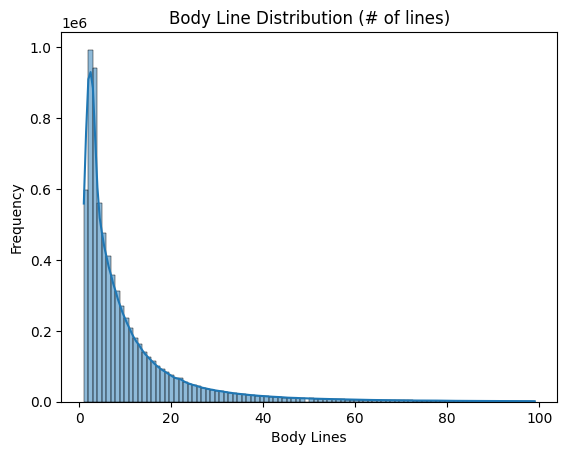
\includegraphics[width=\textwidth]{kapitel4/bodyline.png}
    \end{minipage}\hfill
    \begin{minipage}{0.5\textwidth}
        \centering
        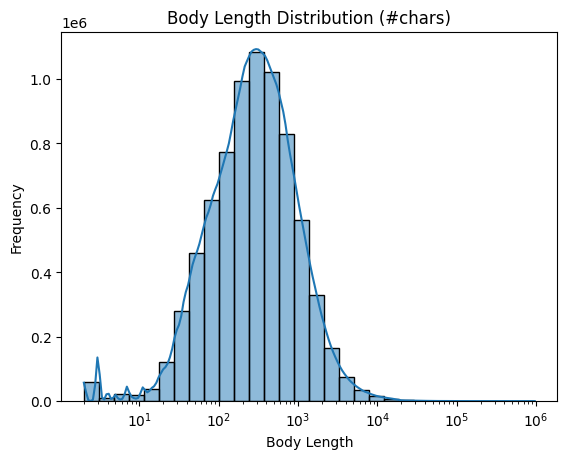
\includegraphics[width=\textwidth]{kapitel4/bodylen.png}
    \end{minipage}
    \caption{Distribution of the number of body lines and body length in TinyFuncData-docstring. The x-axis for the body length distribution is scaled logarithmically.}
    \label{fig:bodydist}
\end{figure}

This version is saved locally as it is the primary version used for training.
Its language distribution is shown in table \ref{tab:final-distribution}.
\begin{table}[h!]
    \centering
    \caption{Language distribution of the final TinyFuncData training set.}
    \begin{tabular}{|>{\raggedright\arraybackslash}m{4cm}|>{\raggedleft\arraybackslash}m{4cm}|>{\raggedleft\arraybackslash}m{4cm}|}
        \hline
        \textbf{Language} & \textbf{Function Count} & \textbf{Percentage (\%)} \\
        \hline
        Total & 6,401,534 & \makebox[\widthof{6,401,534}][r]{100.0000} \\
        \hline
        Python & 3,407,994 & \makebox[\widthof{3,407,994}][r]{53.2371} \\
        \hline
        C & 785,642 & \makebox[\widthof{785,642}][r]{12.2727} \\
        \hline
        C\# & 694,098 & \makebox[\widthof{694,098}][r]{10.8427} \\
        \hline
        Java & 440,217 & \makebox[\widthof{440,217}][r]{6.8767} \\
        \hline
        Ruby & 370,542 & \makebox[\widthof{370,542}][r]{5.7883} \\
        \hline
        JavaScript & 350,351 & \makebox[\widthof{350,351}][r]{5.4729} \\
        \hline
        PHP & 161,854 & \makebox[\widthof{161,854}][r]{2.5284} \\
        \hline
        C++ & 114,124 & \makebox[\widthof{114,124}][r]{1.7828} \\
        \hline
        Shell & 62,993 & \makebox[\widthof{62,993}][r]{0.9840} \\
        \hline
        TypeScript & 13,719 & \makebox[\widthof{13,719}][r]{0.2143} \\
        \hline
    \end{tabular}
    \label{tab:final-distribution}
\end{table}

Figure \ref{fig:language-distributions} shows the percentage changes of each language in relation to the total number of functions for each variant of the dataset.
It can be observed that the most drastic changes occur when filtering by functions with docstring.
The most noticeable change is Python, jumping from under 20\% to over 50\% of data.
Python is perhaps the most prevalent language in \ac{nlp} and \ac{ml} in general.
As will be discussed in chapter \ref{chap:discussion}, Python is also the primary language used for evaluating model code synthesis performance.
This could imply that a lot of Python data found on GitHub is also \ac{ai}-generated, which could also explain why so much Python code has a docstring.
\ac{ai} code is typically heavily commented.
This raises questions about the merit of training a \ac{lm} on \ac{lm}-generated data for this use case, but this topic falls outside the scope of this thesis.

Also notable is that JavaScript and especially Java have a sharp dropoff when filtering for docstrings, with Java dropping by around 15\% and JavaScript by 10\%.
This is surprising, especially considering Java's robust docstring support.

Finally, it should be noted that the ordering of the languages for the original dataset does not match GitHub's ranking from which the languages were selected.
This is most likely due to the fact that some languages are much more function reliant than others.
This may explain some of the previous observations as well -- a language like Java is almost entirely built on functions, and many of them might be simple enough as to need no explicit documentation (like a getter), not to mention main functions.
Languages like Python, which often have logic outside of functions, may have docstrings more commonly as functions are rarer and used more purposefully.
This does not explain why JavaScript, which can also place logic outside of functions, has a steep dropoff as well.

% total amount figure
\begin{comment}
\begin{figure}
    \centering
    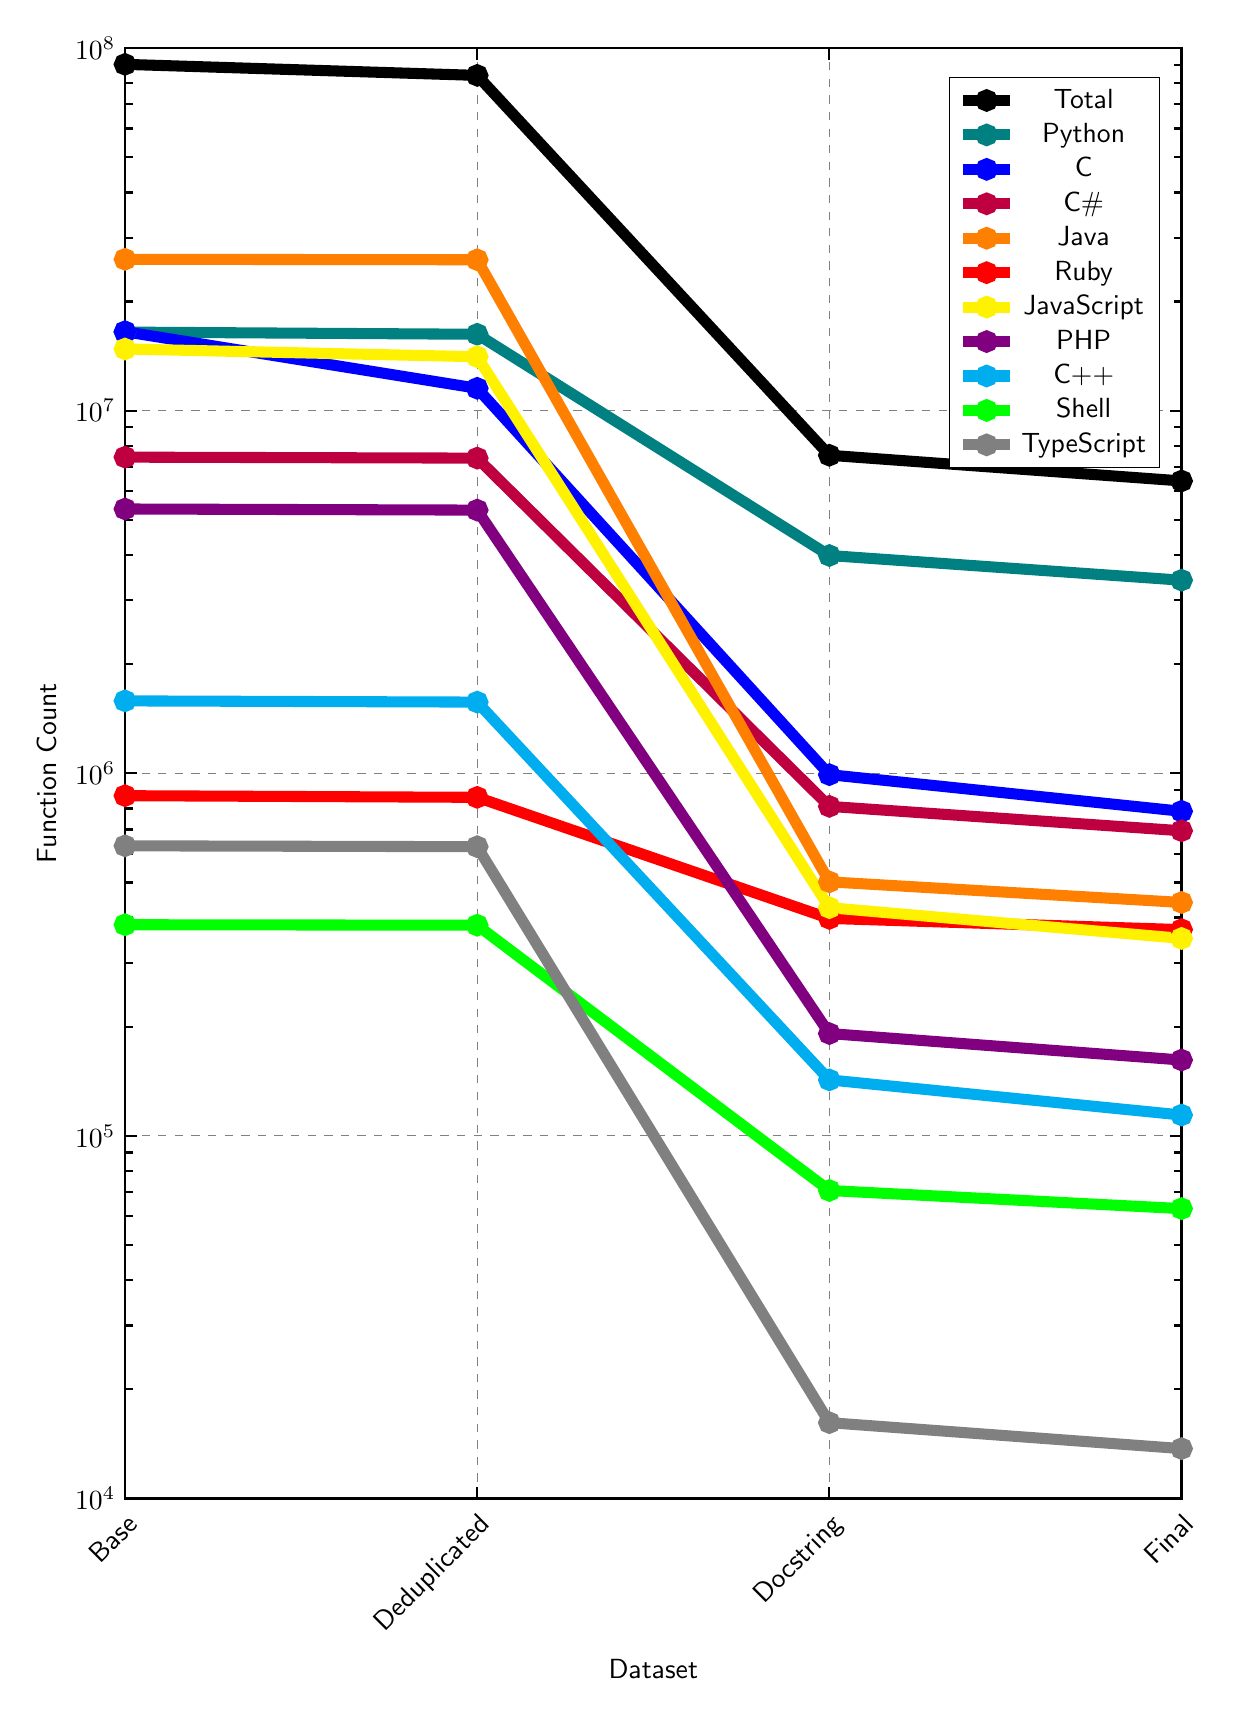
\begin{tikzpicture}
        \begin{axis}[
            width=15cm, height=20cm,
            xlabel={Dataset},
            ylabel={Function Count},
            xtick={1,2,3,4},
            xticklabels={Base, Deduplicated, Docstring, Final},
            xticklabel style={rotate=45, anchor=north east},
            ymode=log,
            log basis y={10},
            ymin=1e4, ymax=1e8,
            grid=major,
            every axis plot/.append style={thick, mark=*, line width=4pt},
            clip=false,
            axis line style={thick, black},
            tick style={thick, black},
            grid style={dashed, gray},
            %legend style={at={(1.05,1)},anchor=north west},
            %legend cell align={left},
            font=\sffamily,
            xmin=1,
            xmax=4
        ]
        % Data for each language
        \addplot[color=black,mark=*] coordinates {(1,90214500) (2,84101961) (3,7535293) (4,6401534)};
        %\node[right] at (axis cs:4.2,6401534) {Total};
        \addlegendentry{Total};
    
        \addplot[color=teal,mark=*] coordinates {(1,16472714) (2,16248323) (3,3987109) (4,3407994)};
        %\node[right] at (axis cs:4.2,3407994) {Python};
        \addlegendentry{Python};
    
        \addplot[color=blue,mark=*] coordinates {(1,16519085) (2,11530315) (3,991275) (4,785642)};
        %\node[right] at (axis cs:4.2,785642) {C};
        \addlegendentry{C};
    
        \addplot[color=purple,mark=*] coordinates {(1,7446313) (2,7400280) (3,810354) (4,694098)};
        %\node[right] at (axis cs:4.2,694098) {C\#};
        \addlegendentry{C\#};

        \addplot[color=orange,mark=*] coordinates {(1,26157106) (2,26077227) (3,501827) (4,440217)};
        %\node[right] at (axis cs:4.2,440217) {Java};
        \addlegendentry{Java};
    
        \addplot[color=red,mark=*] coordinates {(1,867301) (2,858255) (3,397823) (4,370542)};
        %\node[right] at (axis cs:4.2,370542) {Ruby};
        \addlegendentry{Ruby};

        \addplot[color=yellow,mark=*] coordinates {(1,14798610) (2,14088493) (3,425887) (4,350351)};
        %\node[right] at (axis cs:4.2,350351) {JavaScript};
        \addlegendentry{JavaScript};

        \addplot[color=violet,mark=*] coordinates {(1,5356751) (2,5319176) (3,191508) (4,161854)};
        %\node[right] at (axis cs:4.2,161854) {PHP};
        \addlegendentry{PHP};

        \addplot[color=cyan,mark=*] coordinates {(1,1583611) (2,1571530) (3,142663) (4,114124)};
        %\node[right] at (axis cs:4.2,114124) {C++};
        \addlegendentry{C++};

        \addplot[color=green,mark=*] coordinates {(1,382231) (2,380992) (3,70669) (4,62993)};
        %\node[right] at (axis cs:4.2,62993) {Shell};
        \addlegendentry{Shell};

        \addplot[color=gray,mark=*] coordinates {(1,630778) (2,627370) (3,16178) (4,13719)};
        %\node[right] at (axis cs:4.2,13719) {TypeScript};
        \addlegendentry{TypeScript};
        \end{axis}
    \end{tikzpicture}
    \caption{Language distributions among the four versions of the dataset. The y-axis is scaled logarithmically.}
    \label{fig:language-distributions}
\end{figure}
\end{comment}

% percentage amount figure
\begin{figure}[H]
    \centering
    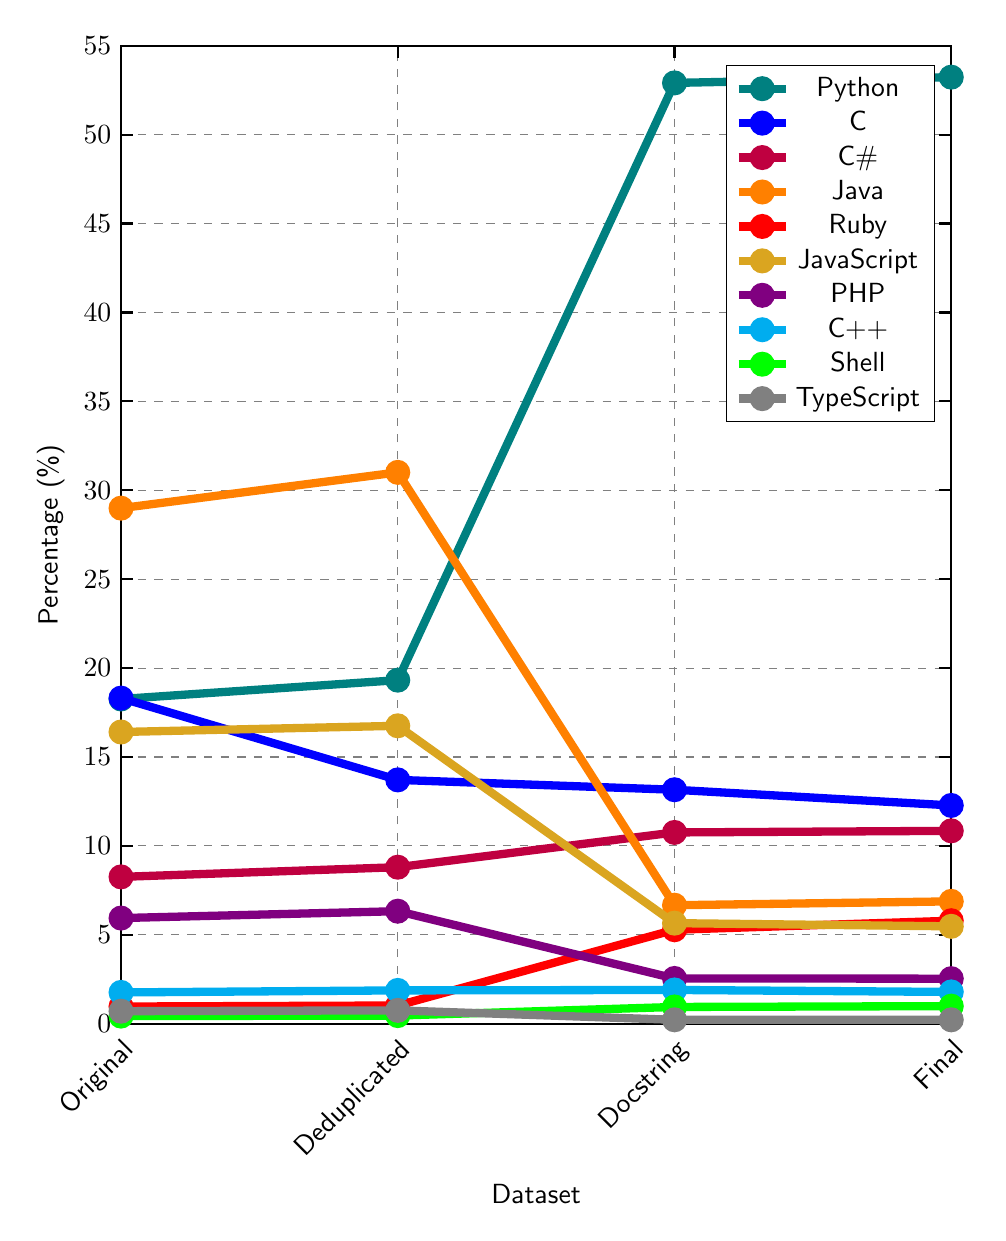
\begin{tikzpicture}
        \begin{axis}[
            width=\textwidth, height=14cm,
            xlabel={Dataset},
            ylabel={Percentage (\%)},
            xtick={1,2,3,4},
            xticklabels={Original, Deduplicated, Docstring, Final},
            xticklabel style={rotate=45, anchor=north east},
            ymode=linear,
            ymin=0, ymax=55,
            xmin=1, xmax=4,
            grid=major,
            every axis plot/.append style={thick, mark=*, line width=3pt},
            clip=false,
            clip mode=individual,
            axis line style={thick, black},
            tick style={thick, black},
            grid style={dashed, gray},
            font=\sffamily
        ]
    
        \addplot[color=teal, mark=*, mark size=3pt] coordinates {(1,18.2595) (2,19.3198) (3,52.9125) (4,53.2371)};
        \addlegendentry{Python};
    
        \addplot[color=blue, mark=*, mark size=3pt] coordinates {(1,18.3109) (2,13.7099) (3,13.1551) (4,12.2727)};
        \addlegendentry{C};

        \addplot[color=purple, mark=*, mark size=3pt] coordinates {(1,8.2540) (2,8.7992) (3,10.7541) (4,10.8427)};
        \addlegendentry{C\#};

        \addplot[color=orange, mark=*, mark size=3pt] coordinates {(1,28.9943) (2,31.0067) (3,6.6597) (4,6.8767)};
        \addlegendentry{Java};

        \addplot[color=red, mark=*, mark size=3pt] coordinates {(1,0.9614) (2,1.0205) (3,5.2795) (4,5.7883)};
        \addlegendentry{Ruby};
    
        \addplot[color=Goldenrod, mark=*, mark size=3pt] coordinates {(1,16.4038) (2,16.7517) (3,5.6519) (4,5.4729)};
        \addlegendentry{JavaScript};
    
        \addplot[color=violet, mark=*, mark size=3pt] coordinates {(1,5.9378) (2,6.3247) (3,2.5415) (4,2.5284)};
        \addlegendentry{PHP};
    
        \addplot[color=cyan, mark=*, mark size=3pt] coordinates {(1,1.7554) (2,1.8686) (3,1.8933) (4,1.7828)};
        \addlegendentry{C++};
    
        \addplot[color=green, mark=*, mark size=3pt] coordinates {(1,0.4237) (2,0.4530) (3,0.9378) (4,0.9840)};
        \addlegendentry{Shell};
    
        \addplot[color=gray, mark=*, mark size=3pt] coordinates {(1,0.6992) (2,0.7460) (3,0.2147) (4,0.2143)};
        \addlegendentry{TypeScript};
    
        \end{axis}
    \end{tikzpicture}
    \caption{Language distributions among the four versions of the dataset.}
    \label{fig:language-distributions}
\end{figure}

\section{Architecture}
\label{sec:architecture}

To finetune a \ac{llm} on a dataset as large as TinyFuncData on limited hardware, many efficiency-boosting tactics have to be used when designing the model and training architecture.
This section will explain the entire architecture for fine-tuning on the TinyFuncData-docstring dataset in detail, explaining all concepts, libraries and parameters used, as well as their purpose.
Many of the libraries used come from the huggingface hub\footnote{\url{https://huggingface.co/} (last visited on 2024-10-31)}, a website focused on hosting \acp{lm}, datasets for model training, \ac{nlp} libraries and documentation, as well as a space for community discussions surrounding the topic.
It hosts over a million models and over 235.000 datasets and is free for anyone to use, download from, and upload their own work to.
\enquote{The hub} will be used interchangably as a shorthand for the full name.

\paragraph{Data Loading:}
The dataset is loaded using the \texttt{load\_dataset()} function from huggingface's \texttt{datasets} library, which can download datasets hosted on the site.
The dataset was saved on the hub during creation, and using this function is the intended way of loading it into a notebook.


\paragraph{Tokenization:}
The \texttt{AutoTokenizer}\footnote{\url{https://huggingface.co/docs/transformers/v4.42.0/en/model_doc/auto\#transformers.AutoTokenizer} (last visited on 2024-10-31)} from huggingface's \texttt{transformers} library is used for tokenization.
\texttt{AutoTokenizer.from\_pretrained()} is used to create a tokenizer for each base model used.
This class automatically loads the appropriate tokenizer for a provided model name.

\paragraph{Configs:}
Two configs are used in order to train the model with \ac{qlora}:
a \texttt{BitsAndBytes\\Config}\footnote{\url{https://huggingface.co/docs/transformers/en/main_classes/quantization\#transformers.BitsAndBytesConfig} (last visited on 2024-10-31)} from \texttt{transformers}, and a \texttt{LoraConfig}\footnote{\url{https://huggingface.co/docs/peft/en/package_reference/lora\#peft.LoraConfig} (last visited on 2024-10-31)} from the \texttt{peft} library.

The \texttt{BitsAndBytesConfig} is used for quantization of models, and it is later passed as an argument when loading the model.
The most important parameters are as follows:
\begin{itemize}
    \item \texttt{load\_in\_4bit} is set to \texttt{True}, causing the model to be 4-bit quantized, as explained in section \ref{sec:qlora}. It does this by replacing the models linear layers with \texttt{bitsandbytes}' quantized layers.
    \item \texttt{bnb\_4bit\_compute\_dtype} is set to \texttt{bfloat16} (brain floating point 16), which changes the computation type, speeding up calculations.
    \item \texttt{bnb\_4bit\_use\_double\_quant} is set to \texttt{True}, causing nested quantization for quantized parameters, saving even more space per parameter.
\end{itemize}

The \texttt{LoraConfig}'s purpose is to turn the model into a \ac{peft} model through the \texttt{get\_peft\_\\model()} function, a model that utilizes \ac{lora}.
The most important parameters are as follows:
\begin{itemize}
    \item \texttt{r}, the rank, is set to 64.
    \item \texttt{lora\_alpha}, used for \ac{lora} parameter scaling, is set to 16. Scaling is used to weigh the new \ac{lora} parameters against the old model parameters. Rank and alpha were decided on after some hyperparameter testing, as explained in section \ref{sec:pretrain}.
    \item \texttt{lora\_dropout} acts like regular dropout and is set to 0.1, a standard value.
\end{itemize}

\paragraph{Model Initialization:}
The different models are loaded using \texttt{transformers}' \texttt{AutoModel\\ForCausalLM.from\_pretrained()}\footnote{\url{https://huggingface.co/docs/transformers/v4.42.0/en/model_doc/auto\#transformers.AutoModelForCausalLM} (last visited on 2024-10-31)}, a class and function designed to easily load pretrained models directly from huggingface for causal language modeling -- predicting the next token given a sequence of tokens.
The most important parameters are as follows:
\begin{itemize}
    \item \texttt{model\_name} is the base models name
    \item \texttt{quantization\_config} takes the \texttt{BitsAndBytesConfig} created earlier.
    \item \texttt{device\_map} is set to \texttt{"auto"} to automatically distribute the model across the server's \acp{gpu}.
\end{itemize}

After initializing the model, \texttt{peft}'s \texttt{prepare\_model\_for\_kbit\_training()} and \texttt{get\_\\peft\_model()} are called to transform the model into a \ac{peft} model.
This is also where the \texttt{LoraConfig} is given to the model.
The first function prepares the model for low-rank training by converting model weights.
The second wraps the model with the new \ac{lora} layers that will be trained, according to the given configuration.

\paragraph{Data Collation:}
for data collation, a \texttt{DataCollatorForLanguageModeling}\footnote{\url{https://huggingface.co/docs/transformers/en/main_classes/data_collator\#transformers.DataCollatorForLanguageModeling} (last visited on 2024-10-31)} from \\\texttt{transformers} is used.
The \texttt{mlm} flag is set to \texttt{False} to disable masked training due to its high resource cost.

\section{Training}
\label{sec:training}

This section describes the training process used to fine-tune the TinyFuncCoder models.
Section \ref{sec:setup} shows the libraries and parameters used in the training pipeline.
Section \ref{sec:hardware} gives a brief explanation of the hardware used for training.
Section \ref{sec:pretrain} describes the various steps in creating the training pipeline, culminating in the final pipeline explained in \ref{sec:finaltrain}.
Figure \ref{fig:architecture} shows a full diagram of the used architecture and training pipeline.
The details of its component are described in section \ref{sec:architecture} as well as the upcoming sections.

\begin{figure}[H]
    \centering
    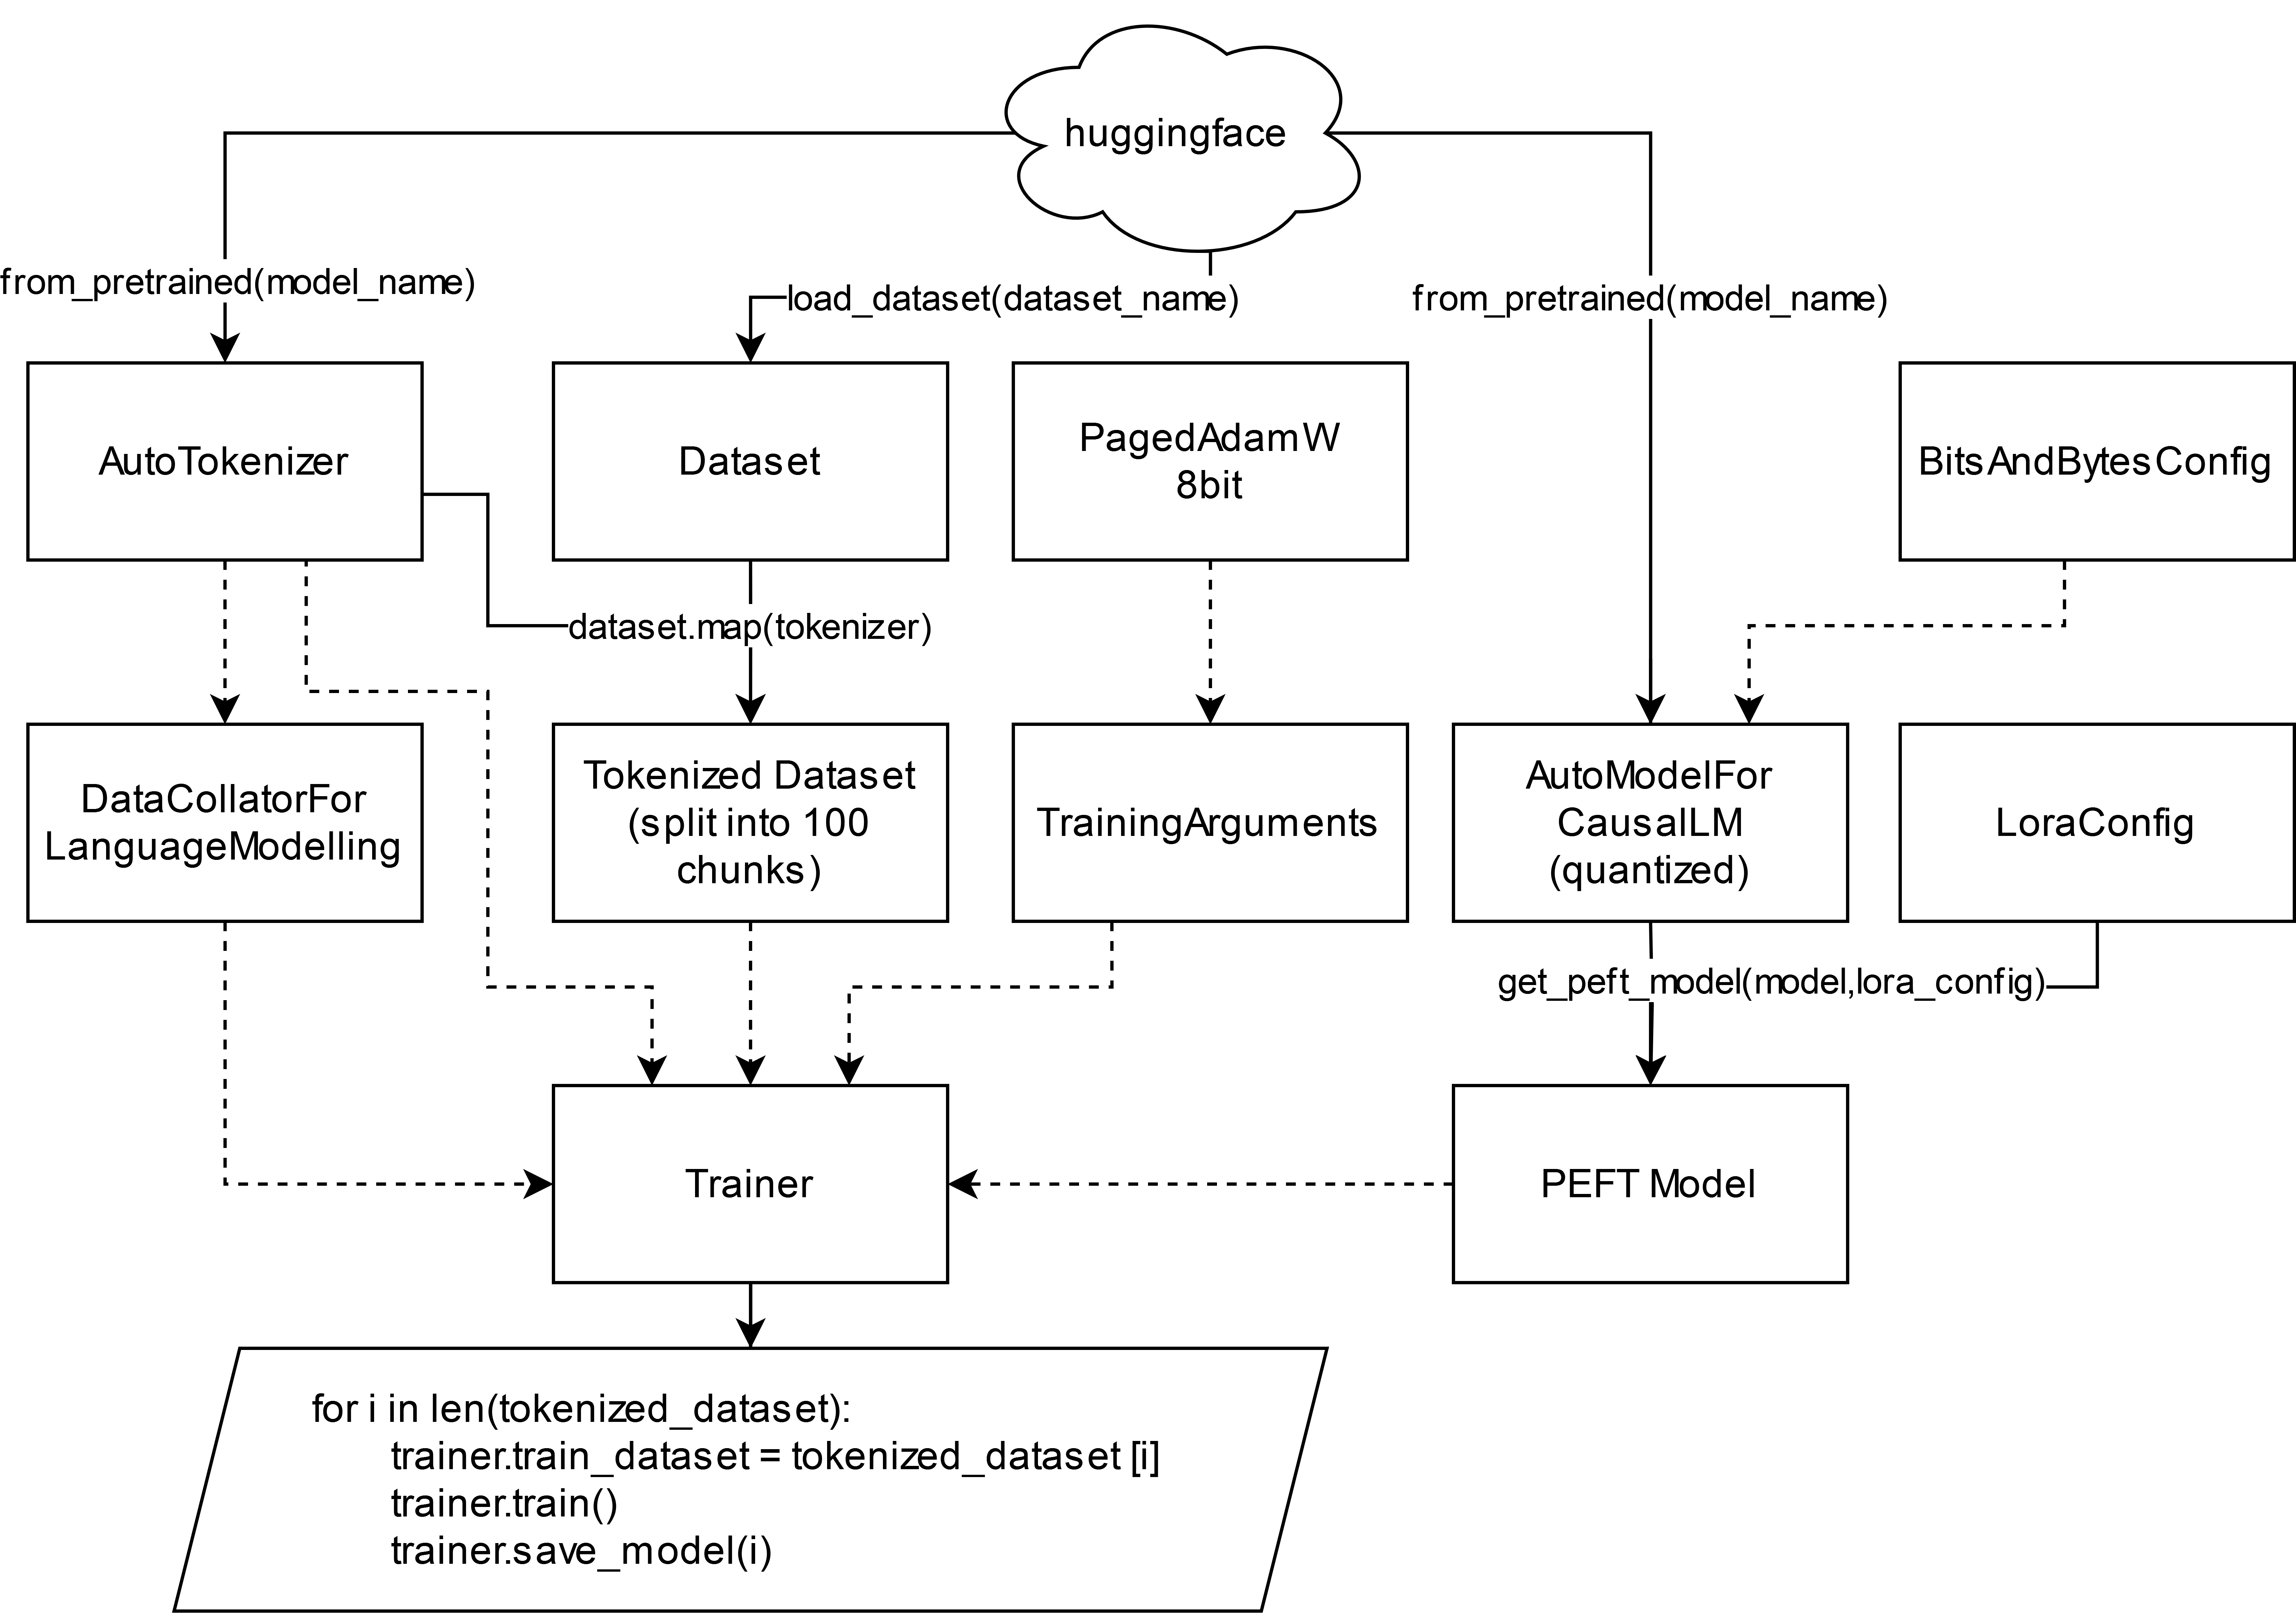
\includegraphics[width=\textwidth]{bilder/kapitel4/architecture.png}
    \caption{The full training pipeline of TinyFuncCoder. Boxes indicate object instances. Solid arrows indicate function calls using the connecting instances. Dotted arrows indicate use of an instance as a variable for another object. Arrows coming from the cloud indicate loading data for instancing from the huggingface hub.}
    \label{fig:architecture}
\end{figure}

\subsection{Training Setup}
\label{sec:setup}
For training the model, \texttt{transformers}' \texttt{Trainer}\footnote{\url{https://huggingface.co/docs/transformers/en/main_classes/trainer\#transformers.Trainer} (last visited on 2024-10-31)} and \texttt{TrainingArguments}\footnote{\url{https://huggingface.co/docs/transformers/en/main_classes/trainer\#transformers.TrainingArguments} (last visited on 2024-10-31)} are used, which allow for easy configuration of a training loop for the model.

\paragraph{Training Arguments:}
The most important training arguments are as follows:
\begin{itemize}
    \item \texttt{per\_device\_\{train/eval\}\_batch\_size}: The batch size for training and evaluation. Both are set to 1, as crashes because of memory issues were the biggest concern during training.
    \item \texttt{gradient\_accumulation\_steps}: The number of steps before a backpropagation is done through the model. This is set to 8 to further reduce memory cost by limiting backpropagation.
    \item \texttt{dataloader\_num\_workers}: This denotes the number of subprocesses to be used in data loading. This is set to 4.
    \item \texttt{learning\_rate}: The learning rate is set to 1e-5.
    \item \texttt{fp16}: Setting this to True will enable 16-bit precision training, rather than the default 32-bit.
    \item \texttt{optim}: The optimizer used by the model. In this case, a PagedAdamW optimizer, which is more memory-efficient than a regular AdamW, is used.
    \item \texttt{\{eval/logging/save\}\_strategy}: is set to \texttt{"steps"} for \texttt{eval}, so that results can be seen at every x training steps. As the dataset is large and training takes long, setting it to \texttt{"epoch"} would not provide sufficient information to monitor and evaluate the training process.
    Important to note is that a step is counted as a backwards pass when using gradient accumulation, so this is only done once each \texttt{\{eval/logging/save\}\_steps $\cdot$ gradient\_accumulation\_steps}. Eval is set to 3200, or half of an epoch, logging arbitrarily to 250, and saving to once per epoch.
    \item \texttt{seed}: The seed used for random number generation, assuring reproducability of the results. It is set to 42.
\end{itemize}

\paragraph{Trainer:}
Finally, to begin training, the \texttt{Trainer} class is initialized with the other objects that have been created so far: the model, training arguments, training and evaluation datasets and the tokenizer and data collator.
Once the trainer has been created, \texttt{trainer.train()} can be called to begin fine-tuning the model.
For TinyLlama, new parameters of around 1.44\% of the total amount of model parameters are trainable using the LoraConfig described earlier.


\subsection{Hardware and Software}
\label{sec:hardware}
Dataset creation, training and evaluation were split between two devices: a personal computer used mainly for filtering the function definitions from The Stack, as well as evaluating the results generated by the models.
Model training, further dataset filtering and result generation was done on a server provided and maintained by Prof. Dr. Oliver Hummel of the faculty of computer science, University of Applied Sciences Mannheim as part of TransforMA\footnote{\url{https://www.hs-mannheim.de/die-hochschule/forschung-und-transfer/transforma.html} (last visited on 2024-31-10)}.
Table \ref{tab:architecture} shows the specs of both machines.

Connection to the TransforMA server was achieved through VS Code's Remote-SSH extension, opening an SSH tunnel to the server.
A VPN connection to the university is also required.
Code was run in VSCode's Jupyter extension.

To prevent having to keep a connection to the server, as it automatically closes after a timeout period, most time intensive tasks were done using papermill\footnote{\url{https://papermill.readthedocs.io/en/latest/} (last visited on 2024-10-31)}.
To this end, the command
\begin{lstlisting}[language=bash]
    nohup papermill notebook.ipynb notebook-out.ipynb 1>>notebook.out 2>> notebook.out &
\end{lstlisting}
is run, executing the notebook using papermill while using nohup to force the code to keep running even when the connection is closed.
1>{}> and 2>{}>, referring to the standard and error output, are saved in <notebook>.out while <notebook>-out.ipynb is a copy of the original notebook that is updated close to real time with the cell outputs.

\begin{table}[!h]
    \centering
    \caption{Specs of the machines used in the creation of TinyFuncCoder and TinyFuncData.}
    \begin{tabular}{l|l|l|l|l}
        \hline
        & \textbf{CPU} & \textbf{RAM} & \textbf{GPU} & \textbf{GPU RAM} \\
        \hline
        \textbf{PC} & $1\times$ AMD Ryzen 5 & 16 GB & $1\times$ NVIDIA GeForce & $1\times$ 8 GB \\
        & 5600X 6-Core & & RTX 3060 Ti & \\
        \hline
        \textbf{TransforMA} & $48\times$ AMD EPYC & 256 GB & $2\times$ NVIDIA GeForce & $2\times$ 24 GB \\
        & 7443P 24-Core & & RTX 4090 & \\
        \hline
    \end{tabular}
    \label{tab:architecture}
\end{table}

\subsection{Exploratory Training}
\label{sec:pretrain}

Creation of the TinyFuncCoder series was an iterative process of testing multiple approaches to maximize model performance within the constraints of the hardware.
The results of the approaches will be more thoroughly presented in section \ref{sec:eval} and only briefly mentioned here to explain decisions made for each iteration.
Every model checkpoint was evaluated on HumanEval and HumanEval+ to compare performance.
While this is not an exhaustive comparison, it is a comparatively quick way to assess model performance, as using multiple metrics would take much longer and slow down the speed of iteration.
HumanEval was chosen as it is the most popular and relatively quick to generate for. It takes around 45 minutes to fully generate all answers, and under a minute to assess them. TinyLlama was chosen for testing because it is the smallest of the models considered (see section \ref{sec:basemodels}) and thus quickest to fine-tune.

The first step to fine-tuning the model was deciding on how to format the functions.
A simple first choice is simply feeding the entire function into the model, in the order \enquote{docstring -- function head -- function body}.
To help the model use appropriate syntax, a custom line is added to the start of the docstring specifying the language in which the function is written.
This simplistic approach quickly proved error-prone, as when using a model trained this way it will not stop generating when the function end is reached, instead generating more comments or functions or even text attempting to explain what the function does.
To stop this behaviour, a start and end token are added before the first and at the end of the last line of all training data.
These are \enquote{<func>} and \enquote{<$\backslash$func>}, similar to opening and closing tags for HTML. 
Tags of a similar form are often used in training.
For example, Gemma uses the pad token \enquote{\texttt{<pad>}}, Magicoder uses \enquote{\texttt{<|end\_of\_sentence|>}} and WizardCoder uses \enquote{\texttt{[PAD]}}.
This way, the model learns a starting point for all functions, the comment clarifying the language, as well as an end point for each of the training functions.
Allowing the model to generate an end token opens the possibility to ignore all generated text past that point, resulting in better results.

Fine-tuning on the entire dataset was not feasible, as even with optimized settings, it was projected to take 300 hours and typically crashed due to memory issues before then.
Instead, multiple subsets of 1\% size were created.
Half of these were done with stratified sampling by language, meaning an equal number of rows for each language, the other half with a fixed size of .1\% of the total per language.
This splitting is done with pandas'
These were split 80/20 into training and validation data, with validation being further split into a valdiation and testing set.
Attempting to use the testing set always resulted in a crash and the second split was eventually deemed unnecessary because the model would be tested on the metrics introduced in \ref{sec:metrics}.
Training and evaluating with these sets of 1\% took around 9.5 hours each for one epoch.
Attempting to train on a 5\% stratified subset also resulted in a crash due to memory issues.

As all of these produced comparably middling results, a next attempt was to fine-tune multiple epochs on a single one of these subsets, which often yielded worse performance. Experimenting with different \ac{lora} parameters also worsened performance on the same data.

This lead to the decision to instead attempt to fine-tune on multiple subsets of the full dataset, swapping each epoch to see more functions to learn from.
Trying to build an architecture to facilitate a single training loop swapping out its dataset for every epoch took four iterations:

For all iterations, a loop was run over the desired epoch count (100).
At this point, the testing set was discarded because it was not being used, increasing the size of the validation set to a full 20\% of the total.
In the first attempt, all relevant classes to the model (tokenizer, training arguments, trainer, model, etc.) were created inside of the training loop.
The dataset was also split at runtime.
At the end of the epoch, a checkpoint was saved, which was used with the trainer's \texttt{resume\_from\_checkpoint} flag to continue training.
However, this changes the training arguments and dataset of the trainer, changing the desired outcome.
Datasets were generated as a stratified sample by language with a seed corresponding to the epoch number.

For the second iteration, most classes were initialized outside of the loop, with only the trainer and dataset being created inside.
This has the desired effect of changing the dataset, but the trainer saves other important values during training which are continuously reset this way.

In the third attempt, the trainer was given a callback function that attempted to change the dataset at the start of each epoch.
This did not work because the trainer kept training before the dataset had time to finish loading.

Finally, the dataset was split into 100 evenly-sized stratified chunks which were saved on disk.
This prevents overlap in the random sampling and allows fast loading because it does not first have to be split at runtime.
The dataset is then simply swapped out through a property call on the trainer at the start of the training loop.
This allows the trainer to be created outside of the loop, retaining its learned properties.
For all iterations, the remnants of dataset loading had to be manually deleted using Python's garbage collection library \texttt{gc}.
A big problem was also setting the training arg's epoch counter.
The issue was that setting an epoch amount of one and saving and resuming from checkpoints did not work because the model thought it was done training (1/1 had been completed).
Setting it higher made the trainer train multiple epochs on the same data.
Previous approaches often could not account for this discrepancy.
Attempts were even made to dynamically alter the epoch counter for every new dataset.
In this fourth iteration, the configuration allows setting the epoch count to one because checkpoints are not being used, solving the issue. With around 9.5 hours per epoch, the total time spent training was around 180 hours, or 7.5 days.

\subsection{Final Training}
\label{sec:finaltrain}

The final training for the TinyFuncCoder series was done on TinyLlama-1.1B-Chat-v1.0 and TinyLlama\_v1.1, resulting in TinyFuncCoder-v1.0 and TinyFuncCoder-v1.1.
All other models on which training was considered (described in section \ref{sec:basemodels}) ran into issues that could not be resolved, including problems with model and data distribution to devices, matrix size mismatches or errors that gave no specific information at all.
Both were trained with the final, successful approach described in section \ref{sec:pretrain}, initially iterating over all 100 chunks of data.
The training was still prone to crashes due to memory issues.
These were consistent and happened at the same points of the same chunks every time, and the offending chunks were simply skipped.
Training was resumed from the most recent checkpoint on the next chunk.
Due to time constraints, training per model was limited to 25 chunks, exactly a quarter of the entire set.
These chunks are 0, 1, 2, 5, 6, 7, 8, 10, 12, 14, 15, 16, 17, 18, 21, 24, 26, 29, 30, 31, 32, 33, 34, 35 and 37, counting up from 0 and skipping all chunks with memory issues. V1.1 additionally skips chunk 21 due to memory issues.
During training for v1.0, a few epochs were erroneously trained starting from the wrong checkpoint.
This was eventually discovered and the model retrained from the proper checkpoint.
Training loss remained close to 1.3 for the entirety of training, as will be more closely examined in \ref{sec:loss}.

Training a single epoch on v1.0, including two evaluations, took around 9.5 hours.
Training v1.1 was initially started with identical parameters, which resulted in a training time of around 2.5 hours.
During this training, the loss jumped to over nine from around two in the third epoch.
Training was restarted, loading the model in 8-bit quantization instead of 4-bit, which improved the loss drastically and prevented it from rapidly increasing, but also increased the training time of an epoch to around twelve hours as much of the \ac{qlora} costs and benefits are reduced with the change to a larger data type.
This puts the total training time for v1.0 to 237.5 hours and for v1.1 to 288 hours, around 10 days and 12 days respectively.
This is ignoring time spent restarting training or the erroneously trained chunks.

\section{Evaluation}
\label{sec:eval}

For the evaluation of the test steps, the EvalPlus GitHub\footnote{\url{https://github.com/evalplus/evalplus} (last visited on 2024-10-31)} repository was downloaded and its code used to generate and evaluate the HumanEval and HumanEval+ benchmarks.
To generate and run the code, a Docker container was used to prevent the potentially harmful code generated by a \ac{lm} to be run without protection.
To this end, VSCode's \ac{wsl} support was used, which in turn connected to Docker Desktop through its built in support for \ac{wsl}.
The command
\begin{lstlisting}[language=bash]
    docker run -v \$(pwd):/app ganler/evalplus:latest --dataset humaneval --samples samples.jsonl
\end{lstlisting}
was used, taken directly from the EvalPlus GitHub page.
To run this command on Windows, \texttt{\$(pwd)} can be swapped for \texttt{\$\{PWD\}}.

For a full evaluation run, the Bigcode Evaluation Harness code\footnote{\url{https://github.com/bigcode-project/bigcode-evaluation-harness} (last visited on 2024-10-31)} was used instead.
It offers a prebuilt evaluation pipeline that allows much customization for how models are loaded, how many generations should be generated, if a peft model is used, if generations should be saved and many more.
This pipeline was used for generating the final outputs for the TinyFuncCoder series, as well as the base TinyLlama models used.
To not have to manually start the generation and evaluation for every model and every metric manually, a notebook was written that has a nested loop for tasks and models and runs the bash command
\begin{lstlisting}[language=bash]
    !accelerate launch main.py --model={name_map[name]} --tasks={eval_type} --save_generations --save_generations_path=save/{name}/{reformatted_path} --n_samples=1 --allow_code_execution --trust_remote_code --prompt=continue --temperature=0.2 --generation_only
\end{lstlisting}

for the base Llama models, or the command

\begin{lstlisting}[language=bash]
    !accelerate launch main.py --model={name_map["llama."+name]} --tasks={eval_type} --save_generations --save_generations_path=save/{name}/{reformatted_path} --peft_model={name_map[name]} --eos="</func>" --n_samples=1 --trust_remote_code --prompt=continue --temperature=0.2 --precision=fp16 --generation_only
\end{lstlisting}

for the TinyFuncCoder series to generate the results.
For evaluation, using Docker containers, the commands are

\begin{lstlisting}[language=bash]
    !docker run -v $(pwd)/{path}:/app/{path}:ro -it evaluation-harness-multiple --model={name_map[name]} --tasks={eval_type} --load_generations_path=/app/{path} --n_samples=1 --allow_code_execution --trust_remote_code --temperature=0.2 --prompt=continue
\end{lstlisting}

and

\begin{lstlisting}[language=bash]
    !docker run -v $(pwd)/{path}:/app/{path}:ro -it evaluation-harness-multiple --model={name_map[name]} --tasks={eval_type} --load_generations_path={path} --n_samples=1 --allow_code_execution --trust_remote_code --temperature=0.2 --peft_model={name_map[name]} --eos="</func>" --precision=fp16 --prompt=continue
\end{lstlisting}

for TinyLlama and TinyFuncCoder respectively.

The specialized call for TinyFuncCoder loads the model as a \ac{peft} model with fp16 rather than fp32 precision, defines its base model and the custom end token \enquote{<$\backslash$func>}.
Further, because TinyFuncCoder expects a certain format for the input (start token, language, docstring, function head), some of the code for getting the problem definitions was altered to reformat it.
All Llama models and all TinyFuncCoder models were evaluated with the base prompt as well as with the reformated prompt.
Evaluation is done with only one sample per problem per model, with a temperature of 0.2 as recommended by previous works \cite{Chen.2021,Luo.2024,Wei.2024}.

For DS-1000, many specific library versions have to be used in support of a deprecated library that is in use.
Because of this, DS-1000 was evaluated last, to prevent potential version conflicts with the other evaluations.
Even when trying to resolve the version conflicts, DS-1000 could not be generated or evaluated with the Bigcode evaluation pipeline.
Instead, a custom generator was written to generate the results, and code taken directly from the DS-1000 GitHub repository\footnote{\url{https://github.com/xlang-ai/DS-1000} (last visited on 2024-10-31)} was taken and altered to evaluate it.

While code was generated for LeetCode with a custom pipeline, no Docker environment is offered to execute this code.
This is unfortunate but makes evaluating the generated code too risky.
The generated files will still be included in the repository.

\section{Code and Repository Structure}
\label{sec:repo}

All code and data created and used by this thesis is made available on GitHub\footnote{\url{https://github.com/JanDiekhoff/Masterarbeit} (last visited on 2024-11-07)} and huggingface\footnote{\url{https://huggingface.co/JanDkff} (last visited on 2024-11-07)}.
The repository is split into six main directories:
\begin{itemize}
    \item \texttt{data} for all code related to dataset creation, including gathering and reuploading, filtering, cleanup, analysis and processing, as well as a parquet copy of the datasets.
    \item \texttt{train} for all code related to training.
    \item \texttt{eval} for all code related to evaluation, including all generated data and altered code from the evaluation metrics.
    \item \texttt{appendix} for all code and data used in the error analysis.
    \item \texttt{thesis} for the \LaTeX code of this thesis.
    \item \texttt{other} for any other code files, mainly test files from the start of the thesis to experiment with the various libraries and other code used.
\end{itemize}